\newpage 

\begin{multicols*}{2}
[\section{Divide And Conquer}]

In divide-and-conquer, we solve a problem recursively, applying three steps at each level of the recursion:
\begin{itemize}
        \item \textbf{Divide} the problem into a number of subproblems that are smaller instances of the same problem.
        \item \textbf{Conquer} the subproblems by solveing them recursively. If the subproblem sizes are small enough, just solve them i a straightforward manner.
        \item \textbf{Combine} the solutions to the subproblems into the solution for the original problem.
\end{itemize}

    When the subproblems are large enough to solve recursively, we call that the \textit{recursive case}. Once the problems become small enough that we no longer recurse, we say that the recursion ``bottoms out'' and that we have gotten down to the \textit{base case}. Sometimes, in addition to ubproblems that are smaller instances of the same problem, we have to solve subproblems that are NOT quite the same as the original problem, and cconsider solvim that problem part of the combine step.

\stepcounter{subsection} % \subsection{The Maximum Subarray Problem}
\stepcounter{subsection} % \subsection{Strassen's Algorithm for Matrix Multiplication}

\subsection{The substitution method for solving recurrences}
The \textit{substitution method} for solving recurrences comprises two steps:

\begin{enumerate}
    \item Guess the form of the solution.
    \item Use the Principle of Mathematical Induction to find the constants and show that the solution works.
\end{enumerate}


    We can use the substitution method to establish either upper or lower bounds on a recurrence. As an example consider the recurrence given by: $T(n) = 2T(\floorfunc{n/2}) + n$. We guess that the solution is $T(n) = O(n\log{n})$. So, we claim that $T(n) \leq cn\log{n}$, for some $c > 0$. Proving the claim would then imply that $T(n) = O(n\log{n})$.
    Using induction, we start by assuming that the bound holds for all positive $m < n$, in particular for $m = \floorfunc{n/2}$, yielding $T(\floorfunc{n/2}) \leq c \floorfunc{n/2} \log(\floorfunc{n/2})$. And substituting into the recurrence yields:

\vspace{-6mm}
\begin{align*}
    T(n) &= 2T(\floorfunc{n/2}) + n \\
         &\leq 2(c \floorfunc{n/2} \log(\floorfunc{n/2})) + n  ~~~~~~~~~~~~~~~~ \textsc{(H.Ind.)} \\
         &\leq cn\log(n/2) + n \\
         &= cn\log{n} + (1 - c\log{2}) n \leq cn\log{n},
\end{align*}
    where the last inequality holds iff $c \geq 1/\log{2}$. To complete the proof we need to check that our solution holds for a base case. That is, we need to show in our case, that we can choose $c$ great enough so that the bound holds for the base case too. 

    This requeriment may lead to problems sometimes. Assume for the sake of the argument that $T(1) = 1$, then the bound $T(n) \leq cn\log{n}$ yields to $T(1) \leq c \cdot 1 \cdot \log{1} = 0$ !!
    We can overcome this by taking advantage of asymptotic definition, requiring us that the bound holds for $n \geq n_0$, for some $n_0 \in \mathbb{N}$.

    \paragraph{Subtleties}
    In almost all cases in which the recurrence has constants or lower-order terms, it will be necessary to \underline{have additional terms} in the upper bound to \underline{cancel out} the constants or lower-order terms. Without the right additional terms, the inductive case of the proof will get stuck in the middle, or generate an impossible constraint; this is a signal to go back to your upper bound and determine what else needs to be added to it that will allow the proof to proceed without causing the bound to change in asymptotic terms.\\

\noindent Consider for example, the following recurrence:

\[
    \begin{cases}
        T(1) = 1, \\
        T(n) = 2T(n - 1) + c_1. \\
    \end{cases}
\] Where $c_1 > 0$ is a constant. Iterating manually on the recurrence ($T(n) = 2\cdot(2 \dotsb ( 2 \cdot (2 \cdot 1 + c_1) + c_1) \dotsb )+ c_1$), we can guess that the solution would be $O(2^n)$.

 We will guess an upper bound of $k 2^n - b$, where $b$ is some constant. We include the $b$ in anticipation of having to deal with the constant $c_1$ that appears in the recurrence relation, and because it does no harm. In the process of proving this bound by induction, we will generate a set of constraints on $k$ and $b$, and if $b$ turns out to be unnecessary, we will be able to set it to whatever we want at the end.

    Our property, then, is $T(n) \leq k2^n - b$, for some two constants $k$ and $b$. Note that this property logically \underline{implies that $T(n)$ is $O(2^n)$}. Let's prove the claim by induction.

The base case $n = 1$ is: $T(1) = 1 \leq k2^1 - b = 2k - b$. This is true as long as $k \geq (b + 1)/2$.
The inductive case: We assume our property is true for $n - 1$. We now want to show that it is true for $n$.

\vspace{-6mm}
\begin{align*}
    T(n) &= 2T(n - 1) + c1 \\ 
         &\leq 2(k2n - 1 - b) + c1 ~~~~ \textsc{(H.Ind)} \\
         &=	k2n - 2b + c1 \\
         &\leq k2n - b
\end{align*} 
This last inequality holds as long as $b \geq c1$. So we end up with two constraints that need to be satisfied for this proof to work, and we can satisfy them simply by letting $b = c_1$ and $k = (b + 1)/2$, which is always possible, as the definition of $O(\cdot)$ allows us to choose any constant. Therefore, we have proved that our property is true, and so $T(n)$ is $O(2^n)$.

Had we not added the lower term $-b$ in the upper bound of $T(n) \leq k 2^n - b$, we could have not proven the bound by induction. Indeed, in the first inequality in the hypothesis of induction we would've got $T(n) \leq 2 k^n  + c_1$, which is $\nleq k 2^n$ 

\paragraph{Changing Variables} Sometimes, a little algebraic manipulation can make an unknown recurrence similar to a known one. Consider for example:
\[
    T(n) = 2T(\floorfunc{\sqrt{n}}) + \log{n}.
\]

Then takign $m = \log{n}$, yields $T(2^m) = 2T(2^{m/2}) + m$. Renaming $S(m) = T(2^m)$, to produce the new recurrence:
\[
    S(m) = 2S(m/2) + m.
\]
We already know $S(m) = O(m\log{m})$, thus $T(n) = T(2^m) = S(m) = O(m\log{m}) = O(\log(n) \cdot \log(\log(n)))$.


\subsection{The Recursion-Tree Method for Solving Recurrences}
Drawing out a recursion tree serves as a straightforward way to devise a good guess. In a \textit{recursion tree}, each node represents the cost of a single subproblem somewhere in the set of recursive function invocations. For example consider the recursion tree for the recurrence $T(n) = 3T(\floorfunc{n/4})  + \Theta(n^2)$. We start by finding an upper bound on the recurrence, and focusing only on asymptotic behavior, assume $4\, |\, n$ and we write $T(n) = 3T(n/4) + cn^2$, for some $c > 0$. The recursion tree for the recurrence would be as follows:

\begin{center}
    \tikzstyle{basic}=[inner sep=4pt]
    \tikzstyle{layer0}=[basic,inner sep=4pt]
    \tikzstyle{layer1}=[basic,inner sep=4pt, node distance=60pt]
    \tikzstyle{layer2}=[basic,inner sep=4pt, node distance=20pt]
    \tikzstyle{leafs}=[basic,inner sep=4pt, node distance=22pt]

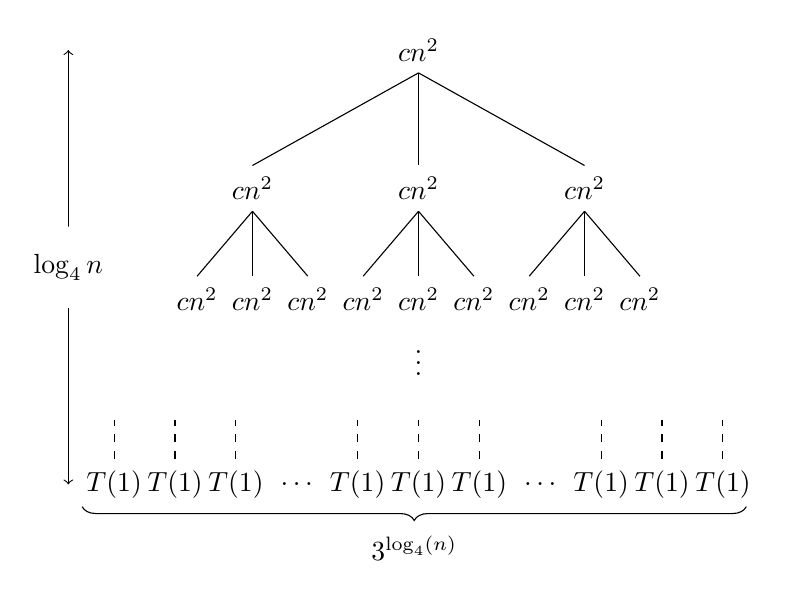
\begin{tikzpicture}
    \node[layer0] (root) at (0,0) {$cn^2$};

    % Layer 0
    \node[layer1] (L1n0) at (0,0) [below of=root, yshift=+10pt]  {$cn^2$};
    \node[layer1] (L1n1) at (0,0) [left of=L1n0]  {$cn^2$};
    \node[layer1] (L1n2) at (0,0) [right of=L1n0] {$cn^2$};

    % Layer 1
    \node[layer2] (L2n0) at (0,0) [below of=L1n0, yshift=-20pt]  {$cn^2$};
    \node[layer2] (L2n1) at (0,0) [left of=L2n0]  {$cn^2$};
    \node[layer2] (L2n2) at (0,0) [right of=L2n0] {$cn^2$};

    \node[layer2] (L2n3) at (0,0) [below of=L1n1, yshift=-20pt]  {$cn^2$};
    \node[layer2] (L2n4) at (0,0) [left of=L2n3]  {$cn^2$};
    \node[layer2] (L2n5) at (0,0) [right of=L2n3] {$cn^2$};

    \node[layer2] (L2n6) at (0,0) [below of=L1n2, yshift=-20pt]  {$cn^2$};
    \node[layer2] (L2n7) at (0,0) [left of=L2n6]  {$cn^2$};
    \node[layer2] (L2n8) at (0,0) [right of=L2n6] {$cn^2$};

    \node[layer2] (dots) at (0,0) [below of=L2n0] {$\vdots$};

    % Leafs
    \node[leafs] (leaf0) at (0,0) [below of=dots, yshift=-25pt] {$T(1)$};
    \node[leafs] (leaf1) at (0,0) [left of=leaf0] {$T(1)$};
    \node[leafs] (leaf2) at (0,0) [right of=leaf0] {$T(1)$};
    \node[leafs] (lowdots0) at (0,0) [left of=leaf1] {$\ldots$};
    \node[leafs] (leaf3) at (0,0) [left of=lowdots0] {$T(1)$};
    \node[leafs] (leaf4) at (0,0) [left of=leaf3] {$T(1)$};
    \node[leafs] (leaf5) at (0,0) [left of=leaf4] {$T(1)$};
    \node[leafs] (lowdots1) at (0,0) [right of=leaf2] {$\ldots$};
    \node[leafs] (leaf6) at (0,0) [right of=lowdots1] {$T(1)$};
    \node[leafs] (leaf7) at (0,0) [right of=leaf6] {$T(1)$};
    \node[leafs] (leaf8) at (0,0) [right of=leaf7] {$T(1)$};

    % Layer 1
    \draw [-]  (root.south) -- (L1n0.north);
    \draw [-]  (root.south) -- (L1n1.north);
    \draw [-]  (root.south) -- (L1n2.north);

    % Layer 2
    \draw [-]  (L1n0.south) -- (L2n0.north);
    \draw [-]  (L1n0.south) -- (L2n1.north);
    \draw [-]  (L1n0.south) -- (L2n2.north);

    \draw [-]  (L1n1.south) -- (L2n3.north);
    \draw [-]  (L1n1.south) -- (L2n4.north);
    \draw [-]  (L1n1.south) -- (L2n5.north);

    \draw [-]  (L1n2.south) -- (L2n6.north);
    \draw [-]  (L1n2.south) -- (L2n7.north);
    \draw [-]  (L1n2.south) -- (L2n8.north);

    % Leafs
    \draw[-,dashed] (leaf0.north) -- ++(0,0.5);
    \draw[-,dashed] (leaf1.north) -- ++(0,0.5);
    \draw[-,dashed] (leaf2.north) -- ++(0,0.5);
    \draw[-,dashed] (leaf3.north) -- ++(0,0.5);
    \draw[-,dashed] (leaf4.north) -- ++(0,0.5);
    \draw[-,dashed] (leaf5.north) -- ++(0,0.5);
    \draw[-,dashed] (leaf6.north) -- ++(0,0.5);
    \draw[-,dashed] (leaf7.north) -- ++(0,0.5);
    \draw[-,dashed] (leaf8.north) -- ++(0,0.5);


    % Annotations and Braces
    \coordinate[right of= root, xshift=-155pt]  (z0) ;
    \coordinate[right of= leaf0, xshift=-155pt]  (z1) ;

    \draw[<->] (z0) -- (z1) node[midway, circle, fill=white, inner sep=1pt] {$\log_4{n}$};

    \coordinate[right of= leaf0, xshift=-150pt]  (y0) ;
    \coordinate[right of= leaf7, xshift=2pt]  (y1) ;
    \draw[decoration={brace,amplitude=5pt,mirror,raise=8pt},decorate]
  (y0) -- node[below=15pt] {$3^{\log_4(n)}$} (y1);

\end{tikzpicture}
\end{center}

The subproblem size for a node at depth $i$ is easily seen to be $n/4^i$. Hence, the problem hits a leaf $n = 1$ when $n/4^i = 1$, that is, $i = \log_4{n}$. Thus the problem has $\log_4{n} + 1$ levels. 

To determine the cost at each level of the three, see that the number of nodes at level $i$ is $3^i$. Since we we reduce by 4 the size of problem each time we go down, the cost of each node at level $i$ is $c(n/4^i)^2$. Adding for all nodes on level $i$, we get the total cost for level $i$ of the tree is $3^i c(n/4^i)^2 = (3/16)^icn^2$. The bottom level has $3^{\log_4(n)} = n^{\log_4{3}}$ nodes, each contributing a cost of $T(1)$. Thus a total cost of $n^{\log_4{3}}T(1) = \Theta(n^{\log_4{3}})$ (assuming $T(1)$ is constant). Adding up all the costs to determine the cost of the entire tree:
\vspace{-4mm}
\begin{align*}
    T(n) &= \sum_{i = 0}^{\log_4(n) - 1} \left(\frac{3}{16} \right)^i + \Theta(n^{\log_4{3}}) \\
         &< \sum_{i = 0}^{\infty} \left(\frac{3}{16} \right)^i + \Theta(n^{\log_4{3}}) \\
         &= \frac{1}{1-(3/16)}cn^2 + \Theta(n^{\log_4{3}}) = \frac{16}{13}cn^2 + \Theta(n^{\log_4{3}}) \\
         &= O(n^2).
\end{align*}
Thus, we have derived a \underline{guess} (not a proof: this was quite $\dots$ informal). This recurrence is indeed $\Theta(n^2)$, which can be easily seen. By the definition of the recurrence it is trivially $\Omega(n^2)$. The bound $O(n^2)$ can be proven by substitution easily.


\subsection{The Master Theorem}
The master method provides a way of solving recurrences of the form $T(n) = aT(n/b) + f(n)$. This recurrence describes the running time of an algorithm that divides a problem of size $n$ into $a$ subproblems, each of size $n/b$. Here $f(n)$ would represent the cost of dividing the problem and combining the results of the subproblems.

\begin{theoremnamed}{Master Theorem}
    Let $a \geq 1$ and $b \geq 1$ be constants, let $f(n)$ be a function, and let $T(n)$ be defined on the nonnegative integers by the recurrence
    \[
        T(n) = aT(n/b) + f(n),
    \]
    where we interpred $n/b$ to mean either $\floorfunc{n/b}$ or $\ceilfunc{n/b}$. Then T(n) has the following asymptotic bounds:
    \begin{enumerate}
        \item If $f(n) = O(n^{\log_b(a) - \epsilon})$ for some constant $\epsilon > 0$, then $T(n) = \Theta(n^{\log_b(a)})$.
        \item If $f(n) =  \Theta(n^{\log_b(a)}$, then $T(n) =  \Theta(n^{\log_b(a)}\log{n})$.
        \item If $f(n) = \Omega(n^{\log_b(a) + \epsilon})$ for some constant $\epsilon > 0$, and if $af(n/b) \leq cf(n)$ for some constant $c < 1$ and all sufficiently large $n$, then $T(n) = \Theta(f(n))$.
    \end{enumerate}
\end{theoremnamed}


As an example consider the recurrence given by $T(n) = 9T(n/3) + n$. For this recurrence, we have $a = 9$, $b = 3$, $f(n) = n$, thus we have that $n^{\log_b{a}} = n^{\log_3{9}} = \Theta(n^2)$. Since $f(n) = O(n^{\log_3{9} - \epsilon})$, where $\epsilon = 1$, we can apply case 1 of the theorem and conclude that $T(n) = \Theta(n^2)$.





\end{multicols*}
